
% \begin{figure}[t] 
% \centering
% % \includegraphics[width=1.0\columnwidth, trim = 0 25 0 0]{Figures/new_fig2.pdf}
% % \includegraphics[width=0.55\columnwidth, trim={0 0 0 23},clip]{Figures/pathlength.pdf}
% 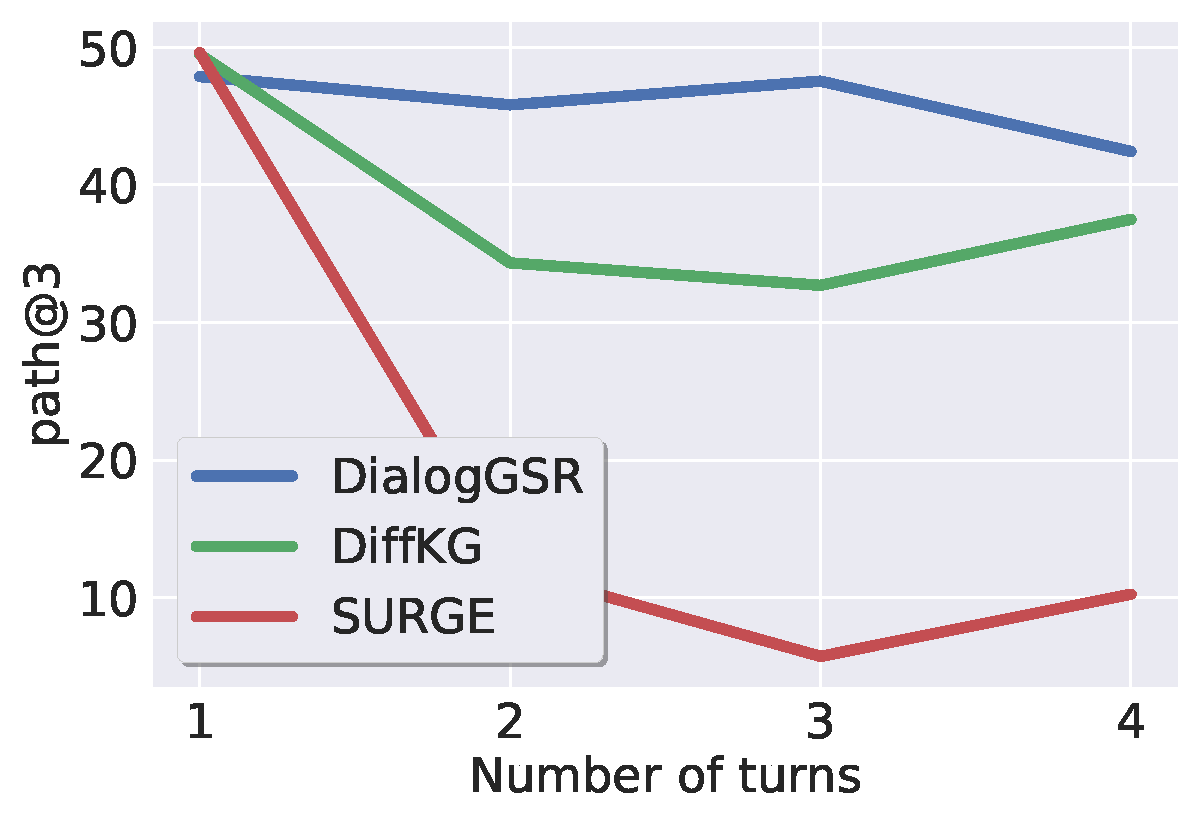
\includegraphics[width=0.55\textwidth]{Figures/turnperform.pdf}
% \caption{Retrieval performance according to the number of turns.}
% \label{fig:anal}
% \end{figure}
\begin{figure}
\small
\centering
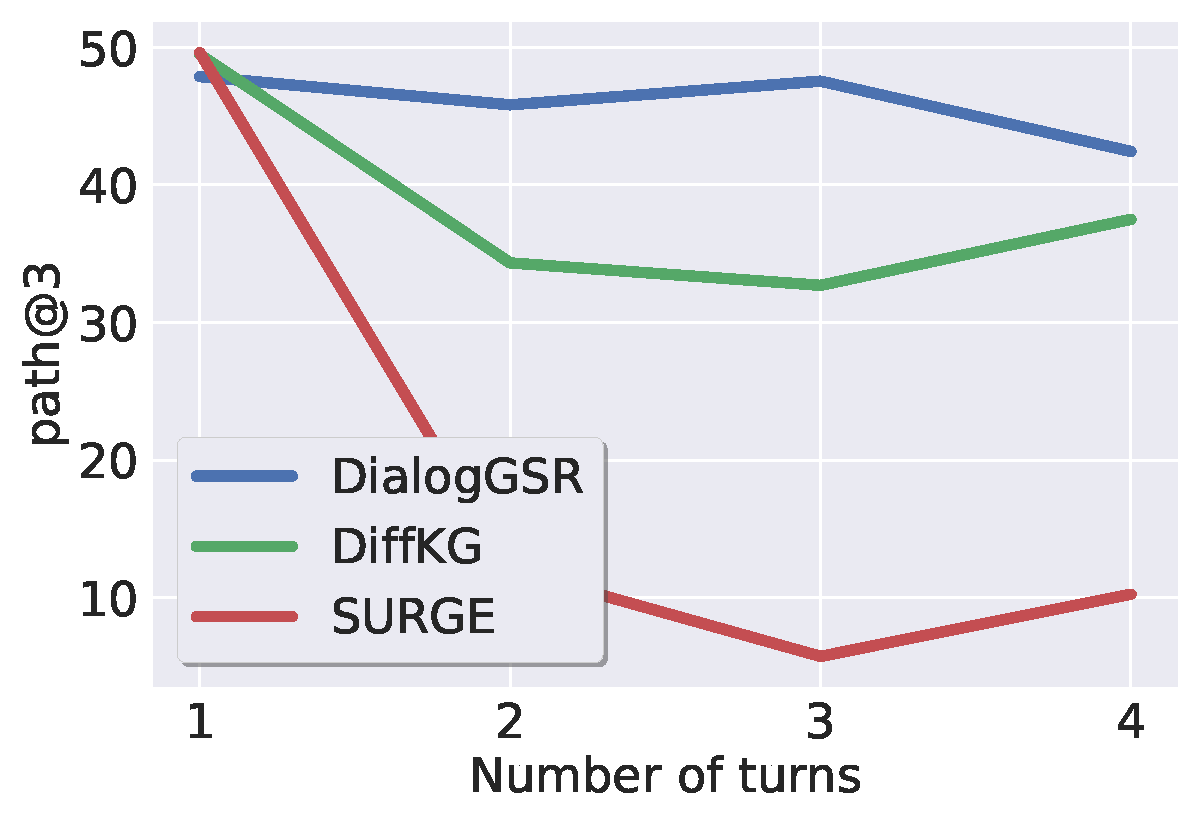
\includegraphics[width=0.8\linewidth]{Figures/turnperform.pdf}
% \vspace{-5pt}
\caption{Retrieval performance according to the number of turns.}
\label{fig:bottleneck}
% \vspace{-13pt}
\end{figure}
\begin{table*}[ht!]
\small
\centering
\resizebox{\textwidth}{!}  
{
    \begin{tabular}{llll}
        \toprule
          Dialog & Gold response & SURGE (Baseline) & DialogGSR (Ours) \\
         \midrule
         \midrule
         \begin{tabular}{@{}l@{}}
(a) Do you like Shaun White?\\
(b) I know he's an Olympic snowboarder he was funny in\\
\quad \ \ Friends With Benefits.\\
(a) Oh, I've never seen that movie, isn't Mila Kunis in it?\\ \quad \ \  I love her! \\
(b) She is. Justin Timberlake and Woody Harrelson were also \\ \quad \ \ in it. Shaun just played a small part. \\
(a) Do you by any chance remember who Mila Kunis is married \\
\quad \ \ too, I totally forgot.\\
\end{tabular}
& 
         \begin{tabular}{@{}l@{}}
She's married to \\ Ashton Kutcher.
\end{tabular} & 
         \begin{tabular}{@{}l@{}}
Mila Kunis is married \\ to Jennifer Lawrence.
\end{tabular} &
\begin{tabular}{@{}l@{}}
Mila Kunis is married \\ to Ashton Kutcher.
\end{tabular}\\         
    \midrule
        \multicolumn{4}{l}{\textit{\textbf{Knowledge triplets $\tau$ retrieved by Baseline}}} \\
        % & \multicolumn{3}{l}{\textit{\textbf{Knowledge triplets $\tau$ retrieved from GSR}}} \\
        \multicolumn{4}{l}{$\langle$ `Justin Timberlake', `place musical career began', `Shelby Forest' $\rangle$} \\
        % & \multicolumn{3}{l}{$\langle$ `Ashton Kutcher', `romantic relationship (with celebrities)', `Mila Kunis' $\rangle$}\\
        \multicolumn{4}{l}{$\langle$ `Justin Timberlake', `place musical career began', `Millington' $\rangle$} \\
        % \multicolumn{3}{l}{$\langle$ `\colorbox{red}{Becca Fitzpatrick}', `write', `\colorbox{yellow}{Silence}'  $\rangle$}\\
        \multicolumn{4}{l}{$\langle$ `Justin Timberlake', `romantic relationship (with celebrities)', `Scarlett Johansson'$ \rangle$} \\
        % \multicolumn{3}{l}{$\langle$ `\colorbox{yellow}{Silence}', `\colorbox{green}{released year}', `\colorbox{cyan}{2012}' $\rangle$}\\
        \midrule
        \multicolumn{4}{l}{\textit{\textbf{Knowledge triplets $\tau$ retrieved by DialogGSR~(ours)}}}\\
        \multicolumn{4}{l}{$\langle$ `Ashton Kutcher', `romantic relationship (with celebrities)', `Mila Kunis' $\rangle$}\\
        \multicolumn{4}{l}{$\langle$ `Friends with Benefits', `starred\_actors', `Mila Kunis'  $\rangle$}\\
        \multicolumn{4}{l}{$\langle$ `Friends with Benefits', `starred\_actors', `Patricia Clarkson' $\rangle$}\\
\bottomrule
\end{tabular}
}
% \vspace{-5pt}
\caption{Comparison on responses generated by SURGE~(Baseline) and DialogGSR given a dialog.}
\label{tab:qual}
% \vspace{-10pt}
\end{table*}

We analyze DialogGSR to answer the following research questions: 
\textbf{[Q1]} Does each component of DialogGSR contribute to a performance improvement? 
\textbf{[Q2]} Are graph-constrained decoding and the entity informativeness score helpful for retrieving context-relevant subgraphs?
\textbf{[Q3]} Is GSR robust to the information bottleneck issue?
\textbf{[Q4]} Is DialogGSR effective with large language models (LLMs)?

\paragraph{Ablation studies.}
We provide the ablation studies to answer \textbf{[Q1], [Q2]} by empirically showing the contribution of each component of DialogGSR in Table~\ref{tab:ablation}.
\textbf{w/o Const.} is generative retrieval without graph-constrained decoding. 
\jyp{\textbf{Hard const.} is the retrieval with graph-constrained decoding but not considering entity informativeness score.}
\textbf{Connection} and \textbf{Katz} use entity informativeness scores based on Connection~($\mathcal{IS}_{\text{con}}$) and Katz metrics~($\mathcal{IS}_{\text{Katz}}$) referred in Section~\ref{sec:3.4}, respectively.
\textbf{with Special tokens (w/o Recon.)} uses special tokens to linearize the knowledge graph without graph reconstruction learning while \textbf{with Special tokens (w/ Recon.)} uses prompts learned with graph reconstruction.
Table~\ref{tab:ablation} shows that each component contributes to the performance improvement of the model.
In particular, graph-constrained decoding is crucial in our generative approach.

In addition, the models with graph constraints show improvements compared to the model without the constraints, which indicates that the graph constraint is important for the generative retrieval of knowledge subgraphs.
Also, using entity informative score~(Connection, Katz) performs better than graph constraints without it since the entity informativeness score reflects graph structural proximity in the decoding process.

\jyp{
\paragraph{Effectiveness of DialogGSR with LLMs.}
To assess the effectiveness of our DialogGSR with Large Language Models~(LLMs)~(\textbf{[Q4]}), we apply it to LLaMA-3~\cite{meta2024introducing}.
The experimental result is shown in Table~\ref{tab:llm}.
From the table, the performance gain of DialogGSR compared to the base model is 2.42 in BLEU-1 score.
In addition, the experimental result demonstrates that our proposed graph-constrained decoding is still important in LLMs. 
This indicates that DialogGSR is also effective in large language models.
}

\paragraph{Information bottleneck issue.}
\jyp{
Information bottleneck issue~\cite{humeau2020poly,lee2022generative} usually occurs when a long text sequence, such as a dialog history, is encoded into a single fixed length of vector.
To explore the robustness of DialogGSR to the information bottleneck issue~(\textbf{[Q3]}), we compare the retrieval performance of DialogGSR with the baselines such as DiffKG and SURGE with respect to the number of turns in dialog histories in Figure~\ref{fig:bottleneck}.
The result shows that DialogGSR is robust for long dialogs whereas the other methods often deteriorate as the number of turns increases.
}


\paragraph{Qualitative analysis.}
\jyp{
We perform qualitative analysis by comparing responses generated from SURGE and DialogGSR.
Table~\ref{tab:qual} shows a sampled \textbf{Gold response} and the responses generated by SURGE~(\textbf{Baseline response}) and DialogGSR~(\textbf{DialogGSR response}) given a multi-turn dialog.
From the table, DialogGSR retrieves more informative knowledge to generate responses compared to the baseline.
Given the last turn ``Do you by any chance remember who Mila Kunis is married too, I totally forgot”, DialogGSR successfully retrieves the knowledge information related to ‘Mila Kunis’ to help provide the appropriate response from the question while the baseline fails to retrieve information related to answer the question. In contrast, the baseline incorrectly retrieves knowledge information related to “Justin Timberlake”, who is mentioned in the past turn (4th turn), which results in a factually incorrect response. This demonstrates that generative retrieval is effective in retrieving informative knowledge and generating knowledge-grounded multi-turn dialogs.
More qualitative results are included in Appendix~\ref{supp:add_qual}.
}